\setchapterpreamble[u]{\margintoc}
\chapter{Statistical models}
\label{chap:statistical_models}

Let us start with the most classical and simplest statistical experiment: the coin toss.
We toss a coin $n$ times, and we model each toss by a random variable in $\{ 0, 1 \}$, where we decide that $1$ means that the toss ended up with heads (so that $0$ means tails).
To each toss is associated a random variable, leading to random variables $X_1, \ldots, X_n$  valued in $\{ 0, 1 \}$, where $X_i$ encodes the outcome of the $i$-th toss.
Each $X_i$ has distribution $\ber(p)$ for $p \in [0, 1]$, where $p$ corresponds to the probability that a coin toss gives heads, namely $\P[X_i = 1]$.%
\sidenote{The notation $\ber(p)$ corresponds to the \emph{Bernoulli} distribution: we will write $X \sim \ber(p)$ whenever $X \in \{ 0, 1\}$ and $\P[X = 1] = p = 1 - \P[X = 0]$.
Another way to obtain a $\ber$ distribution is by setting $X_i = \ind{Y_i \in A}$ where $Y_1, \ldots, Y_n$ are random variables valued in a probability space $(E, \cE)$, with $A \in \cE$, so that $X_i \sim \ber(p)$ with $p = \P[Y_i \in A]$.}
We assume that the $X_i$ are \emph{independent} (since the outcome of the tosses are physically unrelated), and since we are tossing the same coin each time, we assume that these outcomes have the same distribution (meaning that $p$ is constant along the tosses).
Therefore, we assume that $X_1, \ldots, X_n$ are \emph{iid}.%
\sidenote{From now on, iid will stand for \emph{independent and identically distributed}. More about this fundamental assumption will follow.}

\section{Probabilities and statistics} % (fold)
\label{sec:probability_versus_statistics}

Since we assume that the reader is familiar with probability theory, we start this chapter with a comparison between what we do in probabilities and what we do in statistics for the $\ber(p)$ model described above.

\paragraph{Probabilities.} % (fold)

% paragraph probability (end)
In the field of probabilities, we suppose that $p \in (0, 1)$ is known, and we study the properties of the sequence $(X_i)_{i \geq 1}$. 
For instance, we know that the distribution of $S_n = \sum_{i=1}^n X_i$ is $\bin(n, p)$,  
namely that $\P[S_n = k] = \binom{n}{k} p^k (1 - p)^{n-k}$ for $k \in \{0, \ldots, n\}$.%
\sidenote{Where $\binom{n}{k}$ is the $(n, k)$ binomial coefficient given by $\frac{n!}{k! (n - k)!}$.}
It is easy to see that $\E[S_n] = n p$ and that $\var[S_n] = np (1 - p)$, where $\E[\cdot]$ and $\var[\cdot]$ stand respectively for the expectation and the variance.%
\sidenote{The linearity of the expectation gives $\E[S_n] = n \E[X_1] = np$ since the $X_i$ are identically $\ber(p)$ distributed, and, since the $X_i$ are iid, we know that $\var[S_n] = n \var[X_1] = n p (1 - p)$.}%
We can study the asymptotic properties of $S_n$: the law of large number tells us that
\begin{equation*}
	% \label{eq:lln-binomial}
	\frac{S_n}{n} \goas p
\end{equation*}
as $n \go +\infty$ and the central limit theorem tells us by how much we need to normalize $\frac{S_n}{n} - p$ in order to obtain a non-zero limit
\begin{equation*}
	% \label{eq:tcl-binomial}
	\sqrt n \Big(\frac{S_n}{n} - p\Big) \leadsto \nor(0, p(1-p))
\end{equation*}
as $n \rightarrow +\infty$,%
\sidenote{The notation $X_n \goas X$ stands for the \emph{almost sure} convergence of $X_n$ towards $X$ while $X_n \leadsto X$ stands for the convergence of $X_n$ towards $X$ in distribution.}
where $\nor(\mu, \sigma^2)$ stands for the Gaussian distribution with expectation $\mu$ and variance $\sigma^2$.
In the field of probabilities, the object of interest would be the \emph{random variable} $S_n$, that we study knowing the value of $p$.
In particular, if we replace the $\ber(p)$ distribution by the \emph{Rademacher} distribution where $\P[X_i = 1] = 1 - \P[X_i = -1] = p$, the random variable $S_n$ becomes a \emph{random walk} for which many things can be said, depending on the value of $p$.%
\sidenote{But such things are way beyond the topic of this book, let us just cite~\cite{lawler2010random} as a reference on the study of the random walk and its importance in the field of probability theory.}

\paragraph{Statistics.} % (fold)

In statistics, for the $\ber(p)$ example, we don't really care about $S_n$, but we do care about $p$.
We assume that $p$ is \emph{unknown}, and we want to find out things about it.
This objective is called \emph{statistical inference} of the \emph{parameter} $p$.
For instance, we would like to know if $p=1/2$ or not, in order to find out if the coin is well-balanced and not rigged.
The random variables $X_1, \ldots, X_n$ (and $S_n$) live on some probability space $(\Omega, \cA, \P)$, but we don't really care about it either in statistics.
We will always assume, in statistics, that each \emph{observed} outcome $x_i \in \{ 0, 1 \}$ of a coin toss is a \emph{realization} of the random variable $X_i$, namely that
\begin{equation*}
	x_i = X_i(\omega)
\end{equation*}
for some \emph{event} $\omega \in \Omega$.
The realizations $x_i$ are also called \emph{data} or \emph{samples} or \emph{observations}.
But, actually, we will also refer to the random variables $X_i$ in the same way, as \emph{data}, \emph{samples} or \emph{observations}, since we won't manipulate the $x_i$ mathematically,%
\sidenote{nothing can be done with them... it's just deterministic zeros and ones}%
while we will work a lot with the random variables $X_1, \ldots, X_n$.
In statistics, we can do whatever we want with $X_1, \ldots, X_n$ in order to say things about $p$, but we will \emph{never} assume $p$ to be known.%
\sidenote{The parameter $p$ will quickly become a mathematical variable that we will use in equations, in order to perform calculus for instance. Therefore, we will use the specific notation $p_0$ for the ground truth parameter, namely $X_1 \sim \ber(p_0)$, while $p$ will be used as a generic parameter. A statistical parameter will usually be denoted as $\theta$, while the ground truth parameter will be denoted as $\theta_0$ when necessary.}
We will construct measurable functions of $(X_1, \ldots, X_n)$ that do not depend on $p$, these are called \emph{statistics}, in order to tell things about the unknown parameter $p$.
The object of interest in the field of statistics is, therefore, the \emph{distribution of the observations} rather than the observations themselves.


\section{Statistical models and experiences} % (fold)
\label{sec:statistical_models_and_experiences}

Let us consider another very classical problem: the election poll problem, where a population of size $N$ vote for one of two candidates $A$ and $B$.
There are $N_A$ people voting for $A$ while $N - N_A$ vote for $B$, and we want to know about $\theta_0 = N_A / N$.
We perform of poll including $n \ll N$ voters and obtain observations $x_1, \ldots, x_n \in \{ 0, 1 \}$, where $x_i = 1$ (resp. $x_i = 0$) means that voter $i$ votes for $A$ (resp. $B$).
In this problem, both $N_A$ and $N$ are so large that we can suppose that
\begin{equation*} 
	(x_1, \ldots, x_n) = (X_1(\omega), \ldots, X_n(\omega))
\end{equation*}
for some $\omega \in \Omega$, where all $X_i : (\Omega, \cA, \P) \rightarrow (\{0, 1\}, \cP(\{ 0, 1\})$
\marginnote{For a finite set $E$, the notation $\cP(E)$ stands for the $\sigma$-algebra corresponding to the set of all the parts of $E$.}
for $i=1, \ldots,, n$ are such that $X_i \sim \ber(\theta_0)$.
Let's look a little bit at all these mathematical objects. 
In statistics, we are mainly only interested by the fact that the observations are valued in $(\{0, 1\}, \cP(\{ 0, 1\})$ and that the distribution is $\P_{X_i} = \P \circ X_i^{-1} = \ber(\theta_0)$, which is fully described by its parameter $\theta_0 \in (0, 1)$.
Once again, we don't really care about $(\Omega, \cA, \P)$.

\paragraph{Statistical model.}

The \emph{statistical model} for $X = (X_1, \ldots, X_n) \in \{0, 1\}^n$ is the family of distributions
\begin{equation*}
	\big\{ \P_\theta^{\otimes n} : \theta \in (0, 1) \big\}	= \big\{ \ber(\theta)^{\otimes n} : \theta \in (0, 1) \big\},
\end{equation*}
which is a family indexed by $\theta \in (0, 1)$.
The notation $\P^{\otimes n} = \P \otimes \cdots \otimes \P$ stands for the tensor product, namely $\P^{\otimes n}[A_1 \times \cdots \times A_n] = \prod_{i=1}^n \P[A_i]$ for any $A_i \in \cA$, $i=1, \ldots, n$.%
\sidenote{In this book, we will quickly forget to write $\P^{\otimes n}$ and will write simply $\P$ when computations are clear enough, to avoid overloaded notations.}
When we say that this is a statistical model for $X$, we assume that there exist $\theta_0 \in (0, 1)$ such that $X \sim \ber(\theta_0)$.
Once again, let us insist on the following: we do whatever we want with $X_1, \ldots, X_n$ but never with $\theta_0$, which is the unknown parameter.

\paragraph{Another (naive) example.}

Let us consider the problem of the quality of production of screws. 
The dimensions of the screws must satisfy some strong constraints, for instance their length must match quite accurately some fixed size.%
\sidenote{The author of this book does not know anything about screws.}%
\begin{marginfigure}%
	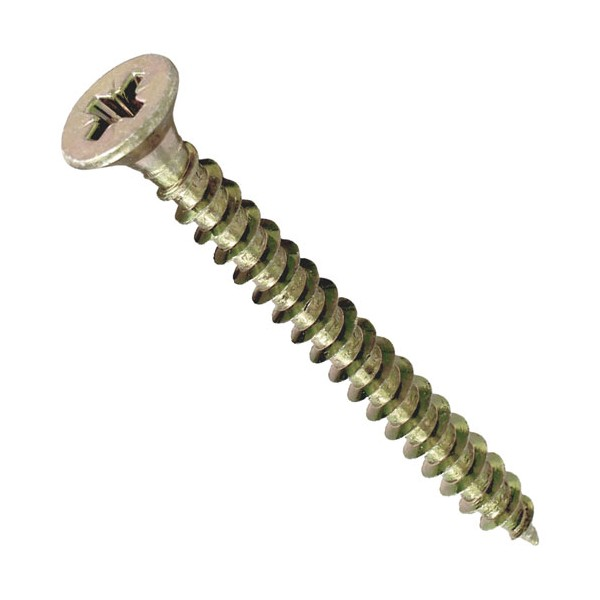
\includegraphics{screw.jpg}%
	\caption{I can't resist the temptation of showing you a screw, so here it is.}%
\end{marginfigure}%
Millions of screws come out of the production chain, and we can't test all of them.
Therefore, we need to assess the production quality by selecting at random a small set of $n$ screws, and we measure their lengths $x_1, \ldots, x_n$.
Since these lengths are highly concentrated around the theoretical desired length $\mu$, and since production errors are usually small, we decide to choose a Gaussian model: we assume that $x_i = X_i(\omega)$ for $X_i \sim \nor(\mu, \sigma^2)$, where $\sigma^2$ corresponds to a variance coming from the (hopefully) small production errors.

\emph{A model is a simplification of the reality.} For this example, we make the following modeling assumptions.
\begin{description}
	\item[Distribution choice.] We choose the distribution $\nor(\mu, \sigma^2)$ for the lengths. So, we implicitly assume that the true underlying distribution of the lengths is \emph{symmetrical} and highly \emph{concentrated} around $\mu$. This may or may not be realistic.%
	\sidenote{A real random variable $X$ is \emph{symmetrical} whenever $\P_X = \P_{-X}$. This means that $\P[X \leq -x] = \P[X \geq x]$ so that $F(-x) = 1 - F(x_-)$ if $F$ is the distribution function of $X$. Also, if $X$ has a density $f$ with respect to the Lebesgue measure, then $f$ is an even function.}
	\item[The iid assumption.] We will assume also that $X_i$ are iid. What this means in practice is that we need to very careful in the way we select the screws coming out of the production lines: for instance, we should pick screws all along a week or a month, at different times, and not all from the same production line, in order to avoid time and machine biases.
\end{description}

Once again, a statistical model is always a simplification and an approximation of the truth.
By \emph{truth} we mean the true distribution $\P_{(X_1, \ldots, X_n)}$ of $(X_1, \ldots, X_n)$.
For instance, the $\nor(0, 1)$ distribution has density $\phi(x) = e^{-x^2/2} / \sqrt{2 \pi}$ supported on $\R$. 
This means that realizations of a $\nor(0, 1)$ distribution can take any value in $\R$, while real samples are usually bounded.
However, we can prove that if $Z \sim \nor(0, 1)$, then $\Phi(x) := \P[Z \leq x]$ satisfies
\begin{marginfigure}
	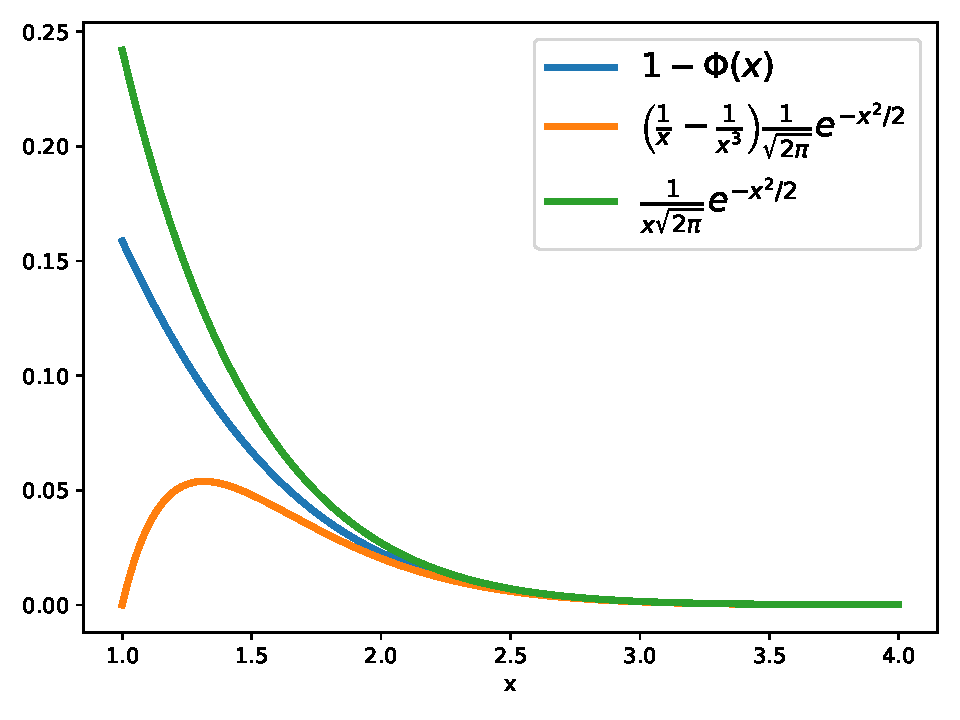
\includegraphics{images/gaussian_queue.pdf}
	\caption{Illustration of the lower and upper bounds proposed in Equation~\eqref{eq:gaussian_queue}.}
\end{marginfigure}%
\begin{equation}
	\label{eq:gaussian_queue}
	\Big( \frac 1x - \frac{1}{x^3} \Big) \frac{1}{\sqrt{2\pi}} e^{-x^2 / 2} \leq 1 - \Phi(x) \leq \frac{1}{x \sqrt{2 \pi}} e^{-x^2 / 2}
\end{equation}
for any $x \geq 1$, which means that the \emph{queue}%
\sidenote{The \emph{queue} of a real random variable $Z$ is the function $x \mapsto \P(Z > x) =: 1 - F_Z(x)$. Whenever $Z \in [0, +\infty)$ almost surely, this function is called also the \emph{survival} function.}%
of the $\nor$ distribution is very tight.
For $x=6$ for instance, we have $\P(Z > x) \leq 10^{-9}$: we will actually never see realizations of $\nor(0, 1)$ outside of $[-6, 6]$, and rarely outside of $[-3, 3]$.
A proof of~\eqref{eq:gaussian_queue} is given in Section~\ref{sec:chap02-proofs} below.
\begin{definition}
	\label{def:statistical_experiment}
	A \emph{statistical experiment} consists of the following two things:
	\begin{itemize}
		\item A \emph{random object} $X$ valued in a measurable space $(E, \cE)$
		\item A \emph{family of distributions} $\cP = \{ P_\theta : \theta \in \Theta\}$ on $(E, \cE)$.
	\end{itemize}
	We suppose that $\P_X = \P \circ X^{-1} \in \cP$, which means that $\P_X = P_{\theta_0}$ for some $\theta_0 \in \Theta$. We say that $\cP$ is a \emph{statistical model} for $X$ and we will denote the statistical experiment as $(X, \cP)$.
	We call $\Theta$ the set of \emph{parameters} of the model.
\end{definition}
\marginnote[*-2]{We call $X$ a \emph{random object} in Definition~\ref{def:statistical_experiment} to stress that it can be a real random variable, a random vector, a random matrix, among other things.
Also, the assumption $\P_X \in \cP$ means that the model is \emph{well-specified}, which is a strong assumption, since it requires that the true distribution belongs to the chosen model $\cP$.}
The random variable $X : (\Omega, \cA, \P) \rightarrow (E, \cE)$ has distribution $\P_X = \P \circ X^{-1}$ which is the probability image of $\P$ by $X$ on $(\Omega, \cA)$.
We will always suppose that there is a family $\{ \P_\theta : \theta \in \Theta\}$ on $(\Omega, \cA)$ that induce $\{ P_\theta : \theta \in \Theta\}$ on $(E, \cE)$ and we will use the notations
\begin{equation*}
	P_\theta[A] = \P_\theta[X \in A] = \P_\theta[ \{ \omega \in \Omega : X(\omega) \in A \}] \quad \forall A \in \cE.
\end{equation*}%
Once again, $(\Omega, \cA, \P)$ is a purely mathematical build of little interest in statistics.
We could even assume that $X$ is the identity function and that $(\Omega, \cA) = (E, \cE)$.
Because of the transfer formula
\begin{equation*}
	\int f(X(\omega)) \P_\theta(d \omega) = \int f(x) P_\theta(dx),
\end{equation*}
we can even work only with $P_\theta$ and forget about $\P_\theta$ and the space $(\Omega, \cA)$.	

We will often work with a set of finite-dimensional parameters $\Theta \subset \R^d$, which corresponds to a \emph{parametric} model, but this space can be more complicated than that (it can be a set of functions with some smoothness properties for instance, such a case is covered by a field called \emph{non-parametric} statistics~\sidecite{tsybakov2008introduction,wasserman2006all}).
We will use the notations
\begin{equation*}
	\E_Q [f(Y)] = \E_{Y \sim Q} [f(Y)] := \int f(y) Q(dy)
\end{equation*}
where we implicitly assume, when computing this expectation, that $Y \sim Q$, and whenever $Q = P_\theta$, we will shorten this notation as follows:
\begin{equation*}
	\E_\theta [f(X)] := \E_{\P_\theta} [f(X)] = \int f(x) P_\theta(dx).
\end{equation*}
We will often work with iid data, namely a \emph{sampled} statistical experiment, as explained in the next definition.
\begin{definition}
A $n$-\emph{sampled} statistical experiment corresponds to data $X = (X_1, \ldots, X_n)$ with $X_i$ iid and $\cP = \{ P_\theta^{\otimes n} : \theta \in \Theta\}$.
\end{definition}
Namely, for a $n$-sampled statistical experiment and $A = \prod_{i=1}^n A_i$, one has the following:
\begin{align*}
	P_\theta^{\otimes n}[A] &= \P_\theta^{\otimes n}[ (X_1, \ldots, X_n) \in A_1 \times \cdots \times A_n] \\
	&= \prod_{i=1}^n \P_\theta[X_i \in A_i] = \prod_{i=1}^n P_\theta[A_i].
\end{align*}
However, we will quickly forget about $n$-sampled experiments and simply say that we observe iid data $X_1, \ldots, X_n$ from a model $\cP = \{ P_\theta \in \Theta \}$ (namely $\P_{X_1} \in \cP$).
\marginnote[*-1]{and when there is little doubt about what we are computing, we will simply forget to write the $\otimes n$ exponents.}

\section{Statistics}
\label{sec:statistics}

We really need at this point to tell the reader what a \emph{statistic} is.%
\begin{definition}
	Given a statistical experiment $(X, \{ P_\theta : \theta \in \Theta \})$, we call \emph{statistic} any measurable function of $X$ that does not depend on~$\theta$.
	A statistic is therefore a quantity that we can compute \emph{using data only}.
\end{definition}
If $X$ is a random variable in $\R^n$ and $S$ a random variable in $\R$, then we know that $S$ is a statistic, namely $S = f(X)$ for some Borel measurable function $f$, if an only if $S$ is $\sigma(X)$-measurable (or simply $X$-measurable).
\sidenote[][*-2]{We recall that $\sigma(X)$ is the $\sigma$-algebra \emph{generated} by $X$, namely $\sigma(X) = X^{-1}(\cB^n)$ where $\cB^n$ is the Borel $\sigma$-algebra of $\R^n$ and note that this statement comes from the Doob lemma: for such $X$ and $S$, we have that $S$ is $X$-measurable if and only if $S = f(X)$ for some Borel measurable function $\R^n \go \R$.}

Now, let us go back to the $\ber(\theta)$ experiment.
Let us first recall that for this experiment we have iid samples $X = (X_1, \ldots, X_n)$, that
$(E, \cE) = (\{0, 1\}^n, \cP(\{0, 1\}^n))$ and that $P_\theta = \ber(\theta)$ with $\Theta = (0, 1)$.
Intuitively, an ``equivalent'' experiment is $S_n := \sum_{i=1}^n X_i$ and $(E, \cE) = (\{ 0, \ldots, n\}, \cP(\{0, \ldots, n\}))$ with $P_\theta = \bin(n, \theta)$ and $\theta \in \Theta = (0, 1)$.
Let us observe that
\begin{equation}
	\label{eq:X_cond_S}
	\begin{split}
	\P_\theta [X_1 = x_1, \ldots, X_n = x_n | S_n = k] &= 
	\frac{\theta^k (1 - \theta)^{n-k}}{\binom{n}{k} \theta^k (1 - \theta)^{n-k}} \\
	&= \frac{1}{\binom{n}{k}}		
	\end{split}
\end{equation}
whenever $x_i \in \{ 0, 1 \}$ for $i=1, \ldots, n$ and $k = \sum_{i=1}^n x_i$, while $\P_\theta [X_1 = x_1, \ldots, X_n = x_n | S_n = k] = 0$ otherwise.
This proves that the \emph{conditional distribution} of $(X_1, \ldots, X_n) | S_n$ \emph{does not depend} on $\theta$.
If we know $S_n$, then we can, \emph{without knowing} $\theta$, build a ``copy'' $X' = (X_1', \ldots, X_n')$ of the original sample $X$, in the sense that $X'$ has the same distribution as $X$.
This is simply achieved, as indicated by Equation~\eqref{eq:X_cond_S}, by choosing the positions of the $S_n = k$ ones (among $n$ ones and zeros) uniformly at random.
This means that $X$ does not bring more information about $\theta$ than $S_n$, and that that $S_n$ is somehow ``sufficient'' from a statistical point of view.
Such a random variable is called a \emph{sufficient statistic}.

For the $\ber(\theta)$ experiment, we will look for statistics of $X$ allowing to infer the unknown parameter $\theta$.
We already now that we can restrict ourselves to statistics of $S_n$ instead of $X$, since $S_n$ is  sufficient.

\section{Identifiable models} % (fold)

The only source of information about $\theta$ available to us about is $X$, through its distribution $P_{\theta}$.
So, in order to infer $\theta$, we need, at least, to be able to recover $\theta$ given $P_\theta$.
We will therefore often require that the model is \emph{identifiable}, as defined below.
\begin{definition}
	We say that a model $\cP = \{ P_\theta : \theta \in \Theta \}$ is \emph{identifiable} whenever the function $\Theta \rightarrow \cP$ given by $\theta \mapsto P_\theta$
	is \emph{injective}.
\end{definition}
Identifiability is a necessary requirement when one wants to perform statistical inference.
If $\theta \mapsto P_\theta$ is not injective, then there is no way to find back $\theta$ from $X \sim P_\theta$.

\begin{example}
	\label{ex:identifiabiliy}
	Obviously, $\theta \mapsto \ber(\theta)$ is injective on $(0, 1)$ and similarly $x \mapsto \ber(\sigmoid(x))$ is injective on $\R$.
	A stupid example is $\mu \mapsto \nor(\mu^2, 1)$ on $\R$, which corresponds to a non-identifiable model.
\end{example}
In Example~\ref{ex:identifiabiliy}, we used the sigmoid function given by $\sigmoid(x) = 1 / (1 + e^{-x})$ for any $x \in \R$.%
\sidenote{The sigmoid function is heavily used in statistics and machine learning, we will come back to it later in the book.}
Identifiability is generally a property that we ensure by choosing and parametrizing correctly the considered statistical model.

However, not all interesting and useful statistical models are identifiable. 
An interesting example of \emph{non-identifiable} model is given by \emph{mixture models}, such as the Gaussian mixture model, where we consider a distribution on $\R^d$ with a density with respect to the Lebesgue measure given by 
\sidenote[][*-4]{The expectations $\mu_k \in \R^d$ correspond to the centroids of the clusters. The covariances $\bSigma_k \in \R^{d \times d}$ are such that $\bSigma_k \succ 0$, which means that $\bSigma_k$ is a positive definite matrix. The matrix $\bSigma_k$ parametrizes the shape of cluster $k$ around $\mu_k$. Finally, the parameters $\pi_k \geq 0$ are such that $\sum_{k=1}^K \pi_k = 1$ and parametrize the relative population of each cluster.}%
\begin{align*}
	f_\theta(x) &= \sum_{k=1}^K \pi_k \phi_{\mu_k, \bSigma_k}(x) \\ 
	&=: \sum_{k=1}^K \frac{\pi_k }{\sqrt{(2 \pi)^d \det (\bSigma_k)}} 
	\exp\Big( -\frac 12 (x - \mu_k)^\top \bSigma_k^{-1} (x - \mu_k) \Big)
\end{align*}
for any $x \in \R^d$, where $\theta = (\pi_k, \mu_k, \bSigma_k)_{k=1, \ldots, K}$ and $K \geq 1$ is an integer corresponding to the number of ``clusters''.
\begin{figure}[htbp]
	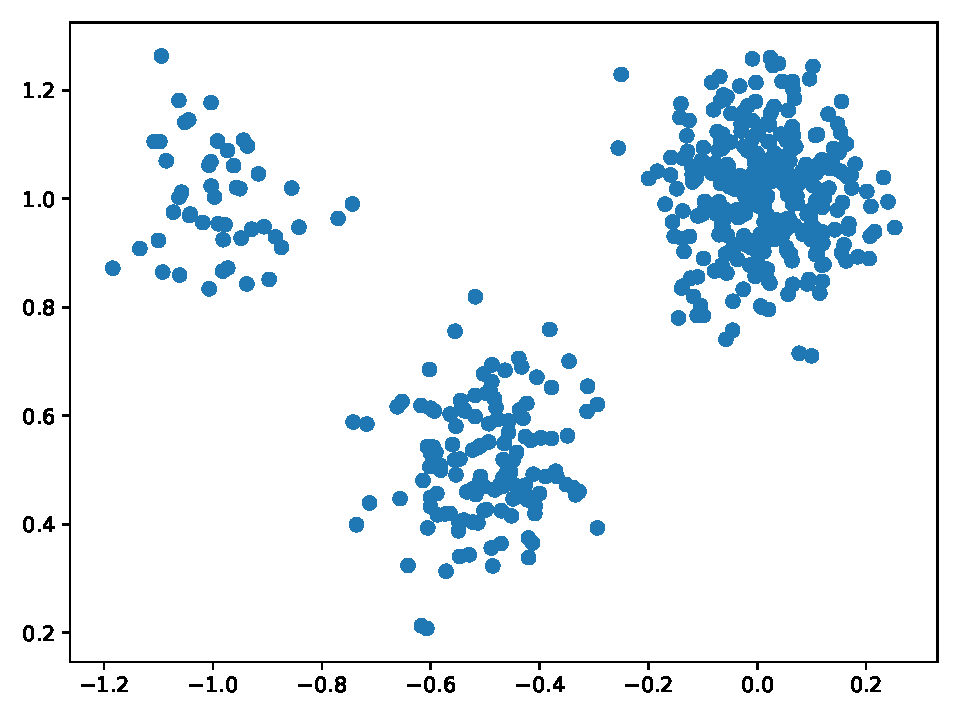
\includegraphics{images/gmm.pdf}
	\caption{$500$ realizations of a Gaussian mixture with $d=2$, $K=3$ $\pi = [\pi_1, \pi_2, \pi_3] = [0.1, 0.6, 0.3]$, $\mu_1 = [-1, 1]$, $\mu_2 = [0, 1]$, $\mu_3 = [-0.5, 0.5]$ and $\bSigma_1 = \bSigma_2 = \bSigma_3 = 0.01 \times \bI_2$.}
\end{figure}
Such a mixture density is non-identifiable, since we have $f_{\theta} = f_{\sigma(\theta)}$
for any permutation $\sigma(\theta) = (\pi_{\sigma(k)}, \mu_{\sigma(k)}, \bSigma_{\sigma(k)})_{k=1, \ldots, K}$ of $\theta$ where $\sigma$ is a permutation of $\{1, \ldots, K \}$.
This simply means that the density distribution $f_\theta$ is invariant by a relabeling of the clusters numbers.
Despite the fact that such a mixture model is not identifiable, it is often used for \emph{model-based clustering}, which is an instance of \emph{unsupervised learning}~\sidecite{murphy2012probabilistic}.
Another family of non-identifiable models is deep neural networks, in which an infinitely large number of parametrizations lead to the same prediction function~\sidecite{goodfellow2016deep}.

\section{Dominated models} 

Whenever $\cP = \{ P_\theta : \theta \in \Theta \}$ with $\Theta \subset \R^d$, we say that $\cP$ is a \emph{parametric} model, since it is parametrized by a finite-dimensional parameter, trivial instances being $\{ \ber(\theta) : \theta \in (0, 1) \}$ for which $d=1$ and $\{ \nor(\mu, v) : (\mu, v) \in \R \times (0, +\infty) \}$ for which $d=2$.
We say that both models are \emph{dominated}, the first being dominated by the counting measure $\nu = \delta_0 + \delta_1$ on $\{ 0, 1\}$,%
\sidenote{The notation $\delta_x$ will stand for the Dirac mass at $x$ which is the probability measure satisfying $\int f(u) \delta_x(du) = f(x)$ for any measurable function $f$.}%
and the second by the Lebesgue measure on $\R$.%
\sidenote{We recall that if $P$ and $Q$ are two finite measures on the same probability space, $P \ll Q$ means that the measure $P$ is \emph{absolutely continuous} with respect to $Q$, namely that $Q(A) = 0 \Rightarrow P(A)= 0$ for any measurable set $A$.}
\begin{definition}
	\label{def:dominated-model}
	We say that a model $\cP = \{ P_\theta : \theta \in \Theta \}$ is dominated if there is a $\sigma$-finite measure $\mu$ such that $P_\theta \ll \mu$ for all $\theta \in \Theta$.
\end{definition}
In Definition~\ref{def:dominated-model}, we require that the dominating measure is $\sigma$-finite, so that we can apply the Radon-Nikodym theorem: since $P_\theta \ll \mu$ for all $\theta \in \Theta$, there is a density 
\begin{equation*}
	f_\theta = \frac{dP_\theta}{d\mu}
\end{equation*}
for all $\theta \in \Theta$, with is unique $\mu$-almost surely.
This means that $P_\theta[A] = \int f_\theta(x) \mu(dx)$ for any measurable set $A$.%
\marginnote{Let us recall the Radon-Nikodym theorem. Let $P$ be a probability and $Q$ be a $\sigma$-finite measure on a measurable space $(\Omega, \cA)$ and assume that $P \ll Q$. Then, there is a non-negative random variable $L$ such that $P[A] = \int_\Omega L(\omega) \ind{A}(\omega) Q(d \omega)$ for any $A \in \cA$. We denote $L = dP / dQ$ and $L$ is unique $Q$-almost surely.}
This domination property allows to work with densities instead of distributions: a model can be therefore defined as a family of densities $\{ f_\theta : \theta \in \Theta \}$ together with a dominating measure (which is in most cases the Lebesgue measure, a counting measure, or a combination of both.)
\begin{example}
	Let us consider the \emph{zero-inflated Laplace distribution}, which is a distribution on $\R$ given by
	\begin{equation*}
		P_\theta(dx) = \pi_0 \delta_0(dx) + (1 - \pi_0) \frac{\lambda}{2} e^{-\lambda |x|} dx
	\end{equation*}
	for $\theta = (\pi_0, \lambda) \in \Theta = (0, 1) \times (0, +\infty)$, which is dominated by the measure $\mu = \delta_0 + \leb$, where $\leb$ stands for the Lebesgue measure on $\R$.
\end{example}
\marginnote[*-4]{The notation $P(dx) = f(x) dx$ means that the distribution $P$ has density $f$ with respect to the Lebesgue measure.}%
Non-dominated models are usually pathological and uninteresting examples, such as the model
\begin{equation*}
	P_\theta = \frac 1e \sum_{n \in \N} \frac{1}{n!} \delta_{\theta n}
\end{equation*}
for $\theta \in (0, +\infty)$, which cannot be dominated by a $\sigma$-finite measure.

% Let us finish this chapter with an example of non-parametric model: we observe $X_1, \ldots, X_n$ with a density $f \in F$ with respect to the Lebesgue measure, where $F$ is the set of probability densities on $[0, 1]^d$ that are $C^2$ and such that $\grad^2 f(x) \mleq L \bI_d$.%
% \sidenote{The notation $\nabla^2 f(x)$ stands for the Hessian matrix of $f$, while $\bI_d$ is the identity matrix on $\R^d$. Finally, for two symmetric matrices $\bA$ and $\bB$, the notation $\bA \mleq \bB$ means $\bB - \bA \mgeq 0$, namely that $\bB - \bA$ is a symmetric and positive semi-definite matrix.}%
% In such a setting, we work with an infinite dimensional set of parameters $F$, and need to build a \emph{non-parametric} estimator of the unknown density $f$.

\section{Proofs} % (fold)
\label{sec:chap02-proofs}

\begin{proof}[Proof of Inequalities~\eqref{eq:gaussian_queue}]
	The upper bound is just easily obtained using
\begin{equation*}
	1 - \Phi(x) = \frac{1}{\sqrt{2 \pi}} \int_{x}^{+\infty} e^{-t^2 / 2} dt \leq \frac{1}{\sqrt{2 \pi}} \int_{x}^{+\infty} \frac{t}{x} e^{-t^2 / 2} dt = \frac{e^{-x^2 / 2}}{x \sqrt{2 \pi}} 
\end{equation*}
while the lower bound comes from the fact that
\begin{equation*}
	\int_{x}^{+\infty} \Big(1 - \frac{3}{t^4} \Big) e^{-t^2 / 2} dt = \Big( \frac{1}{x} - \frac{1}{x^3} \Big) e^{-x^2 / 2}
\end{equation*}
which concludes the proof.
\end{proof}
